\documentclass[a4paper,14pt]{extarticle}
\usepackage[utf8]{inputenc}
\usepackage[T1]{fontenc}
\usepackage[russian]{babel}
\usepackage{amsmath, amssymb}
\usepackage{geometry}
\geometry{left=2cm, right=2cm, top=2cm, bottom=2cm}
\usepackage{hyperref}
\hypersetup{
	colorlinks=true,
	linkcolor=black,
	urlcolor=blue,
}
\usepackage{newtxtext, newtxmath}
\usepackage{longtable}
\usepackage{makecell}
\usepackage{graphicx}
\usepackage{indentfirst}

\begin{document}
	
	% Титульный лист
	\begin{titlepage}
		\centering
		{\large Федеральное автономное образовательное учреждение высшего образования «Национальный исследовательский университет ИТМО»}
		
		\vspace{1cm}
		
		{\large Факультет Программной инженерии и компьютерной техники}
		
		\vspace{2cm}
		
		{\large Дисциплина: «Физика»}
		
		\vspace{0.5cm}
		
		{\large Лабораторная работа №1}
		
		{\large Исследование распределения случайной величины}
		
		\vfill
		
		\raggedleft
		{\large Выполнил:}
		
		{\large Студент группы P3213 Ушаков Роман Павлович}
		
		\vspace{0.5cm}
		
		{\large Преподаватель:}
		
		{\large Дыкова Анастасия Вадимовна}
		
		\vspace{4.5cm}
		
		\centering
		\large Санкт-Петербург, 2026
	\end{titlepage}
	
	\tableofcontents
	\newpage
	
	\section{Цели работы}
	Исследование распределения случайной величины на примере многократных измерений определенного интервала времени.
	
	\newpage
	\section{Задание}
	\begin{enumerate}
		\item Провести многократные измерения определенного интервала времени.
		\item Построить гистограмму распределения результатов измерения.
		\item Вычислить среднее значение и дисперсию полученной выборки.
		\item Сравнить гистограмму с графиком функции Гаусса с такими же как и у экспериментального распределения средним значением и дисперсией.
	\end{enumerate}
	
	\newpage
	\section{Ход работы}
	
	\subsection{Основные расчётные формулы}
	
	Для обработки результатов использовались следующие соотношения:
	\begin{itemize}
		\item среднее арифметическое (выборочное среднее):
		\[
		\langle t \rangle_N = \frac{1}{N} \sum_{i=1}^{N} t_i;
		\]
		\item выборочное среднеквадратичное отклонение:
		\[
		\sigma_N = \sqrt{\frac{1}{N-1} \sum_{i=1}^{N} \left( t_i - \langle t \rangle_N \right)^2};
		\]
		\item опытная плотность вероятности для каждого интервала гистограммы:
		\[
		\frac{\Delta N_i}{N \Delta t};
		\]
		\item теоретическая плотность нормального распределения (функция Гаусса):
		\[
		\rho(t) = \frac{1}{\sigma_N \sqrt{2\pi}} \exp\left( -\frac{(t - \langle t \rangle_N)^2}{2\sigma_N^2} \right);
		\]
		\item максимальное значение плотности нормального распределения:
		\[
		\rho_{\max} = \frac{1}{\sigma_N \sqrt{2\pi}}.
		\]
	\end{itemize}
	
	\newpage
	\subsection{Результаты измерений}
	
	В таблице~\ref{tab:data} приведены результаты 50 измерений заданного промежутка времени цифровым секундомером. Для каждого измерения указано отклонение от среднего и квадрат отклонения.
	
	\begingroup
	\renewcommand{\arraystretch}{1.6}
	\begin{longtable}{|c|c|c|c|}
		\caption{Результаты прямых измерений}
		\label{tab:data}\\ \hline
		№ & $t_i$, с & $\Delta t_i = t_i - \langle t \rangle_N$, с & $(\Delta t_i)^2$, с$^2$ \\ \hline
		\endfirsthead
		
		\multicolumn{4}{c}{Продолжение таблицы~\ref{tab:data}} \\ \hline
		№ & $t_i$, с & $\Delta t_i$, с & $(\Delta t_i)^2$, с$^2$ \\ \hline
		\endhead
		
		\hline
		\endfoot
		
		\hline
		\endlastfoot
		
		1  & 9,68  & 0,013  & 0,000169 \\ \hline
		2  & 8,98  & -0,687 & 0,471969 \\ \hline
		3  & 9,83  & 0,163  & 0,026569 \\ \hline
		4  & 9,08  & -0,587 & 0,344569 \\ \hline
		5  & 8,73  & -0,937 & 0,877969 \\ \hline
		6  & 9,70  & 0,033  & 0,001089 \\ \hline
		7  & 10,16 & 0,493  & 0,243049 \\ \hline
		8  & 9,73  & 0,063  & 0,003969 \\ \hline
		9  & 9,76  & 0,093  & 0,008649 \\ \hline
		10 & 10,16 & 0,493  & 0,243049 \\ \hline
		11 & 10,23 & 0,563  & 0,316969 \\ \hline
		12 & 10,21 & 0,543  & 0,294849 \\ \hline
		13 & 9,68  & 0,013  & 0,000169 \\ \hline
		14 & 9,71  & 0,043  & 0,001849 \\ \hline
		15 & 9,91  & 0,243  & 0,059049 \\ \hline
		16 & 9,06  & -0,607 & 0,368449 \\ \hline
		17 & 9,76  & 0,093  & 0,008649 \\ \hline
		18 & 10,36 & 0,693  & 0,480249 \\ \hline
		19 & 9,91  & 0,243  & 0,059049 \\ \hline
		20 & 10,45 & 0,783  & 0,613089 \\ \hline
		21 & 9,78  & 0,113  & 0,012769 \\ \hline
		22 & 9,91  & 0,243  & 0,059049 \\ \hline
		23 & 10,10 & 0,433  & 0,187489 \\ \hline
		24 & 9,90  & 0,233  & 0,054289 \\ \hline
		25 & 9,83  & 0,163  & 0,026569 \\ \hline
		26 & 9,50  & -0,167 & 0,027889 \\ \hline
		27 & 9,96  & 0,293  & 0,085849 \\ \hline
		28 & 9,90  & 0,233  & 0,054289 \\ \hline
		29 & 9,80  & 0,133  & 0,017689 \\ \hline
		30 & 9,66  & -0,007 & 0,000049 \\ \hline
		31 & 10,25 & 0,583  & 0,339889 \\ \hline
		32 & 10,01 & 0,343  & 0,117649 \\ \hline
		33 & 9,46  & -0,207 & 0,042849 \\ \hline
		34 & 9,88  & 0,213  & 0,045369 \\ \hline
		35 & 10,43 & 0,763  & 0,582169 \\ \hline
		36 & 9,96  & 0,293  & 0,085849 \\ \hline
		37 & 9,95  & 0,283  & 0,080089 \\ \hline
		38 & 10,18 & 0,513  & 0,263169 \\ \hline
		39 & 8,73  & -0,937 & 0,877969 \\ \hline
		40 & 8,86  & -0,807 & 0,651249 \\ \hline
		41 & 9,56  & -0,107 & 0,011449 \\ \hline
		42 & 9,48  & -0,187 & 0,034969 \\ \hline
		43 & 8,76  & -0,907 & 0,822649 \\ \hline
		44 & 9,18  & -0,487 & 0,237169 \\ \hline
		45 & 9,23  & -0,437 & 0,190969 \\ \hline
		46 & 8,88  & -0,787 & 0,619369 \\ \hline
		47 & 8,88  & -0,787 & 0,619369 \\ \hline
		48 & 9,80  & 0,133  & 0,017689 \\ \hline
		49 & 9,48  & -0,187 & 0,034969 \\ \hline
		50 & 8,96  & -0,707 & 0,499849 \\ \hline
		& $\langle t \rangle_N = 9{,}667$ с & $\sum \Delta t_i = 0{,}000$ с & \makecell{$\sigma_N = 0{,}476$ \\  $\rho_{\max} = 0{,}838$ с$^{-1}$} \\ \hline
	\end{longtable}
	\endgroup
	
	\newpage
	\subsection{Данные для построения гистограммы}
	
	Диапазон значений \(t_{\min} = 8{,}73\) с, \(t_{\max} = 10{,}45\) с.  
	Выбрано число интервалов \(m = 7 \approx \sqrt{50}\).  
	Ширина интервала \(\Delta t = 0{,}25\) с.  
	Границы интервалов: 8,70; 8,95; 9,20; 9,45; 9,70; 9,95; 10,20; 10,45.
	
	В таблице~\ref{tab:hist} приведены границы интервалов, число результатов, попавших в каждый интервал, опытная плотность вероятности, середины интервалов и теоретические значения плотности нормального распределения.
	
	\begingroup
	\renewcommand{\arraystretch}{1.6}
	\begin{table}[h!]
		\centering
		\caption{Данные для построения гистограммы}
		\label{tab:hist}
		\begin{tabular}{|c|c|c|c|c|}
			\hline
			Границы интервалов, с & $\Delta N$ & $\dfrac{\Delta N}{N \Delta t}$, с$^{-1}$ & t, с & $\rho$, с$^{-1}$ \\ \hline
			$[8{,}70; 8{,}95)$ & 6  & 0,48 & 8,825 & 0,176 \\ \hline
			$[8{,}95; 9{,}20)$ & 5  & 0,40 & 9,075 & 0,387 \\ \hline
			$[9{,}20; 9{,}45)$ & 1  & 0,08 & 9,325 & 0,647 \\ \hline
			$[9{,}45; 9{,}70)$ & 8  & 0,64 & 9,575 & 0,822 \\ \hline
			$[9{,}70; 9{,}95)$ & 16 & 1,28 & 9,825 & 0,793 \\ \hline
			$[9{,}95; 10{,}20)$& 8  & 0,64 & 10,075& 0,581 \\ \hline
			$[10{,}20; 10{,}45]$& 6  & 0,48 & 10,325& 0,323 \\ \hline
		\end{tabular}
	\end{table}
	\endgroup
	
	\newpage
	\subsection{Проверка нормальности распределения}
	
	Для количественной проверки близости экспериментального распределения к нормальному вычислим границы стандартных интервалов \(\pm \sigma\), \(\pm 2\sigma\), \(\pm 3\sigma\) и определим долю результатов, попавших в каждый интервал. Полученные значения сравним с теоретическими вероятностями для нормального распределения.
	
	\begingroup
	\renewcommand{\arraystretch}{1.6}
	\begin{table}[h!]
		\centering
		\caption{Проверка нормальности распределения}
		\label{tab:norm}
		\begin{tabular}{|c|c|c|c|c|c|}
			\hline
			 & от, с & до, с & \(\Delta N\) & \(\Delta N / N\) & \(P\) \\ \hline
			\(\langle t \rangle_N \pm \sigma\) & 9,191 & 10,143 & 30 & 0,60 & 0,683 \\ \hline
			\(\langle t \rangle_N \pm 2\sigma\) & 8,714 & 10,620 & 50 & 1,00 & 0,954 \\ \hline
			\(\langle t \rangle_N \pm 3\sigma\) & 8,238 & 11,096 & 50 & 1,00 & 0,997 \\ \hline
		\end{tabular}
	\end{table}
	\endgroup
	
	Как видно из таблицы, для интервала \(\pm 1\sigma\) экспериментальная доля (0,60) несколько ниже теоретической вероятности (0,683). Для интервалов \(\pm 2\sigma\) и \(\pm 3\sigma\) все результаты попали в соответствующие интервалы, что формально даёт доли 1,00 против теоретических 0,954 и 0,997. Это объясняется ограниченным объёмом выборки (\(N = 50\)) и отсутствием «хвостов» распределения за пределами \(2\sigma\) в данной серии измерений.
	
	\begin{figure}[h!]
		\centering
		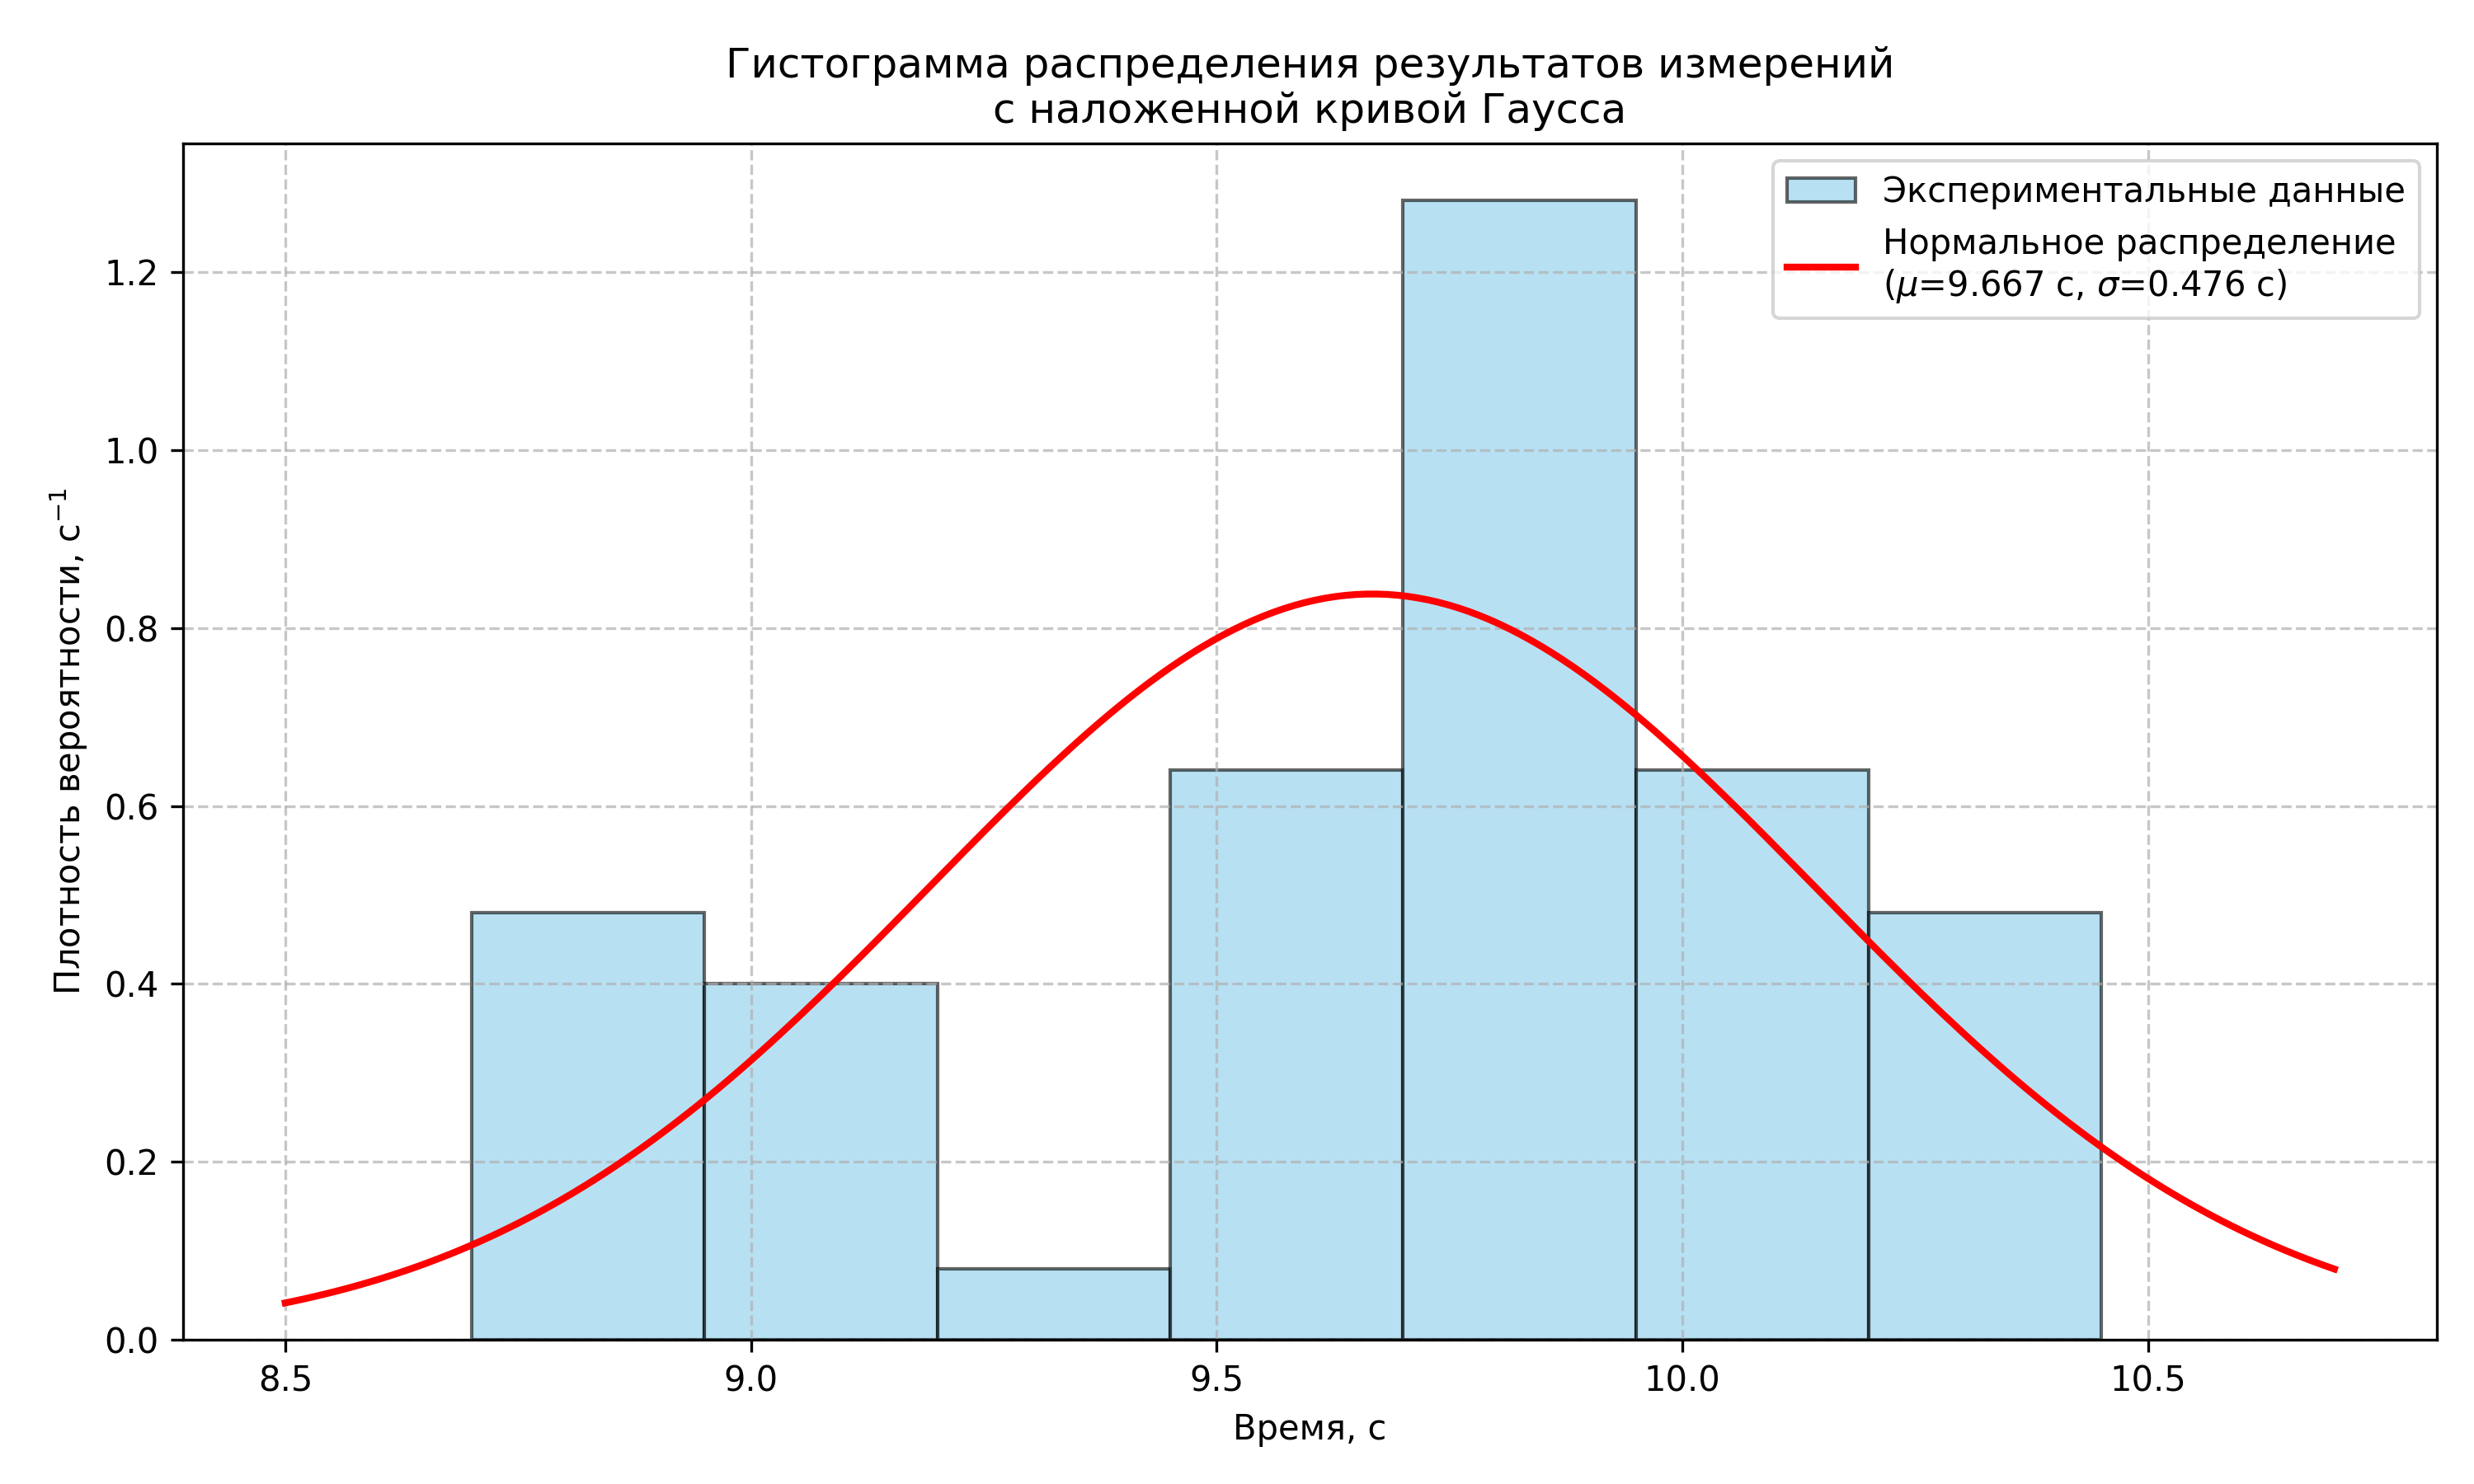
\includegraphics[width=0.85\textwidth]{lab1_chart.png}
		\caption{Гистограмма распределения результатов измерений с наложенной кривой нормального распределения}
		\label{fig:hist}
	\end{figure}
	
	\newpage
	\section{Вывод}
	
	В ходе данной лабораторной работы мы провели многократные измерения заданного интервала времени с помощью цифрового секундомера и исследовали распределение полученных значений. По результатам измерений и вычислений была построена гистограмма, кооторая согласуется с кривой нормального распределения. 
	
	Таким образом, мы убедились, что результаты измерений случайной величины (времени, задаваемого человеком) подчиняются закону, близкому к нормальному.
	
\end{document}